\section{Top-$k$ Single Term Frequency}

\begin{Definition}
  Given a query term (or phrase) $q$ of length $m$ and a parameter $k$. Report the \defi{top-$k$ documents with respect to single term frequency}{Top-$k$ Single Term Frequency}.
\end{Definition}

\begin{Theorem}
  \label{thm:singleTermFrequencySimple}
  The top-$k$ documents can be found in time $\mathcal{O}(m + x(\log k + \log N))$, where $x$ is the number of distinct documents $q$ appears in.
\end{Theorem}

\begin{Proof}
  The documents can be found in the following steps:
  \begin{enumerate}
    \item Get the $x$ distinct documents $d_{r_1}, \ldots, d_{r_x}$ where $q$ occurs in using the method from Section~\ref{sec:documentListing} in $\mathcal{O}(m)$.
    % TODO (pjungeblut): How can this be done in O(log N)? Find out and add here.
    \item Determine the frequency $f_{d_{r_i},q}$ of $q$ in each $d_{r_i}$. This can be done in $\mathcal{O}(\log N)$ per document.
    \item Maintain a min-heap of $(f_{d_{r_i},q}, d_{r_i})$-pairs of size $k$. The heap operations take time $\mathcal{O}(\log k)$.
  \end{enumerate}
  In total we get $\mathcal{O}(m + x \cdot \log N + x \cdot \log k) = \mathcal{O}(m + x(\log k + \log N))$.
\end{Proof}

The solution presented in Theorem~\ref{thm:singleTermFrequencySimple} is already independent of the text length $n$. However it is still dependent on $x$, which can in the worst case be as large as the number of documents $N$.

% TODO (pjungeblut): Add space requirement to the theorem.
\begin{Theorem}
  The top-$k$ documents can be found in time $\mathcal{O}(m \cdot t_{LF} + \log n\cdot k)$ (Gog \cite{Gog2015}).
\end{Theorem}

\begin{Proof}
  We will prove this theorem with a running example: Consider the concatenation $C = \texttt{ATA\#TAAA\#TATA\#\$}$ of length $n=15$ consisting of three documents. The first step is to build the generalized suffix tree \id{GST} of~$C$. It is shown in Figure~\ref{fig:singleTermFrequencySuffixTree}. A document id~$i$ is added to an inner node~$v$, if~$v$ is the lowest common ancestor of two leaves marked by~$i$. These document ids are shown in red.

  \begin{figure}[htb]
    \centering
    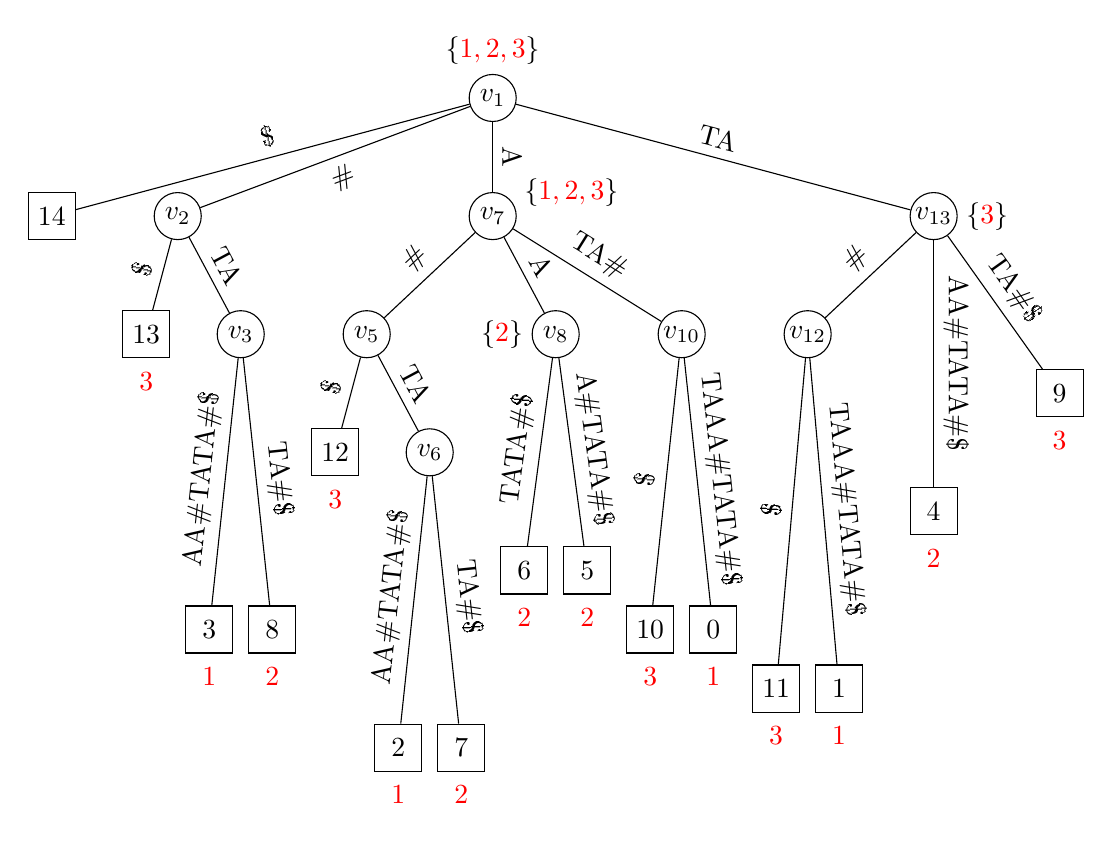
\begin{tikzpicture}[x={(4mm, 0mm)}, y={(0mm, 15mm)}]
  \tikzstyle{vertex}=[draw, minimum size=17pt, inner sep=0pt]

\node[vertex, circle] (v1) at (1, 0) {$v_1$};
\node (l1) at (1, 0.4) {$\{{\color{red}1,2,3}\}$};

\node[vertex, circle] (v2) at (-9, -1) {$v_2$};
\draw (v1) -- (v2) node[below, sloped, pos=0.5] {\#};

\node[vertex, circle] (v3) at (-7, -2) {$v_3$};
\draw (v2) -- (v3) node[above, sloped, pos=0.5] {TA};

\node[vertex, circle] (v7) at (1, -1) {$v_7$};
\node (l7) at (3.5, -0.8) {$\{{\color{red}1,2,3}\}$};
\draw (v1) -- (v7) node[above, sloped, pos=0.5] {A};

\node[vertex, circle] (v5) at (-3, -2) {$v_5$};
\draw (v7) -- (v5) node[above, sloped, pos=0.5] {\#};

\node[vertex, circle] (v6) at (-1, -3) {$v_6$};
\draw (v5) -- (v6) node[above, sloped, pos=0.5] {TA};

\node[vertex, circle] (v8) at (3, -2) {$v_8$};
\node (l8) at (1.3, -2) {$\{{\color{red}2}\}$};
\draw (v7) -- (v8) node[above, sloped, pos=0.5] {A};

\node[vertex, circle] (v10) at (7, -2) {$v_{10}$};
\draw (v7) -- (v10) node[above, sloped, pos=0.5] {TA\#};

\node[vertex, circle] (v13) at (15, -1) {$v_{13}$};
\node (l13) at (16.7, -1) {$\{{\color{red}3}\}$};
\draw (v1) -- (v13) node[above, sloped, pos=0.5] {TA};

\node[vertex, circle] (v12) at (11, -2) {$v_{12}$};
\draw (v13) -- (v12) node[above, sloped, pos=0.5] {\#};

\node[vertex] (s14) at (-13, -1) {$14$};
\draw (v1) -- (s14) node[above, sloped, pos=0.5] {\$};

\node[vertex] (s13) at (-10, -2) {$13$};
\node (d13) at (-10, -2.4) {${\color{red}3}$};
\draw (v2) -- (s13) node[above, sloped, pos=0.5] {\$};

\node[vertex] (s3) at (-8, -4.5) {$3$};
\node (d3) at (-8, -4.9) {${\color{red}1}$};
\draw (v3) -- (s3) node[above, sloped, pos=0.5] {AA\#TATA\#\$};

\node[vertex] (s8) at (-6, -4.5) {$8$};
\node (d8) at (-6, -4.9) {${\color{red}2}$};
\draw (v3) -- (s8) node[above, sloped, pos=0.5] {TA\#\$};

\node[vertex] (s12) at (-4, -3) {$12$};
\node (d12) at (-4, -3.4) {${\color{red}3}$};
\draw (v5) -- (s12) node[above, sloped, pos=0.5] {\$};

\node[vertex] (s2) at (-2, -5.5) {$2$};
\node (d2) at (-2, -5.9) {${\color{red}1}$};
\draw (v6) -- (s2) node[above, sloped, pos=0.5] {AA\#TATA\#\$};

\node[vertex] (s7) at (0, -5.5) {$7$};
\node (d7) at (0, -5.9) {${\color{red}2}$};
\draw (v6) -- (s7) node[above, sloped, pos=0.5] {TA\#\$};

\node[vertex] (s6) at (2, -4) {$6$};
\node (d6) at (2, -4.4) {${\color{red}2}$};
\draw (v8) -- (s6) node[above, sloped, pos=0.5] {TATA\#\$};

\node[vertex] (s5) at (4, -4) {$5$};
\node (d5) at (4, -4.4) {${\color{red}2}$};
\draw (v8) -- (s5) node[above, sloped, pos=0.5] {A\#TATA\#\$};

\node[vertex] (s10) at (6, -4.5) {$10$};
\node (d10) at (6, -4.9) {${\color{red}3}$};
\draw (v10) -- (s10) node[above, sloped, pos=0.5] {\$};

\node[vertex] (s0) at (8, -4.5) {$0$};
\node (d0) at (8, -4.9) {${\color{red}1}$};
\draw (v10) -- (s0) node[above, sloped, pos=0.5] {TAAA\#TATA\#\$};

\node[vertex] (s11) at (10, -5) {$11$};
\node (d11) at (10, -5.4) {${\color{red}3}$};
\draw (v12) -- (s11) node[above, sloped, pos=0.5] {\$};

\node[vertex] (s1) at (12, -5) {$1$};
\node (d1) at (12, -5.4) {${\color{red}1}$};
\draw (v12) -- (s1) node[above, sloped, pos=0.5] {TAAA\#TATA\#\$};

\node[vertex] (s4) at (15, -3.5) {$4$};
\node (d4) at (15, -3.9) {${\color{red}2}$};
\draw (v13) -- (s4) node[above, sloped, pos=0.5] {AA\#TATA\#\$};

\node[vertex] (s9) at (19, -2.5) {$9$};
\node (d9) at (19, -2.9) {${\color{red}3}$};
\draw (v13) -- (s9) node[above, sloped, pos=0.5] {TA\#\$};

\end{tikzpicture}

    \caption{The generalized suffix tree for concatenation $C = \texttt{ATA\#TAAA\#TATA\#\$}$. The red numbers on the leaves are the document array. The red marks on the inner vertices show the lowest common ancestor of two equal elements in the document array (as in document listing in Section~\ref{sec:documentListing}).}
    \label{fig:singleTermFrequencySuffixTree}
  \end{figure}

  In the next step the nodes need to be numbered. For each inner node~$v$ assign it the identifier $\id{id}(v)$ which is the index of the rightmost leaf in the leftmost subtree of~$v$ plus~$1$. This numbering has the following properties:
  \begin{enumerate}
    \item $\id{id}(v) \neq \id{id}(w)$ for all $v \neq w$. To show that this is true, we need to distinguish two cases: Assume $\proc{LCA}(v,w) \not\in \{v,w\}$. Then they have disjoint subtrees, so they get a different id. If however $\proc{LCA}(v,w) \in \{v,w\}$, then w.l.o.g. $v$ is in $w$'s subtree. But if they got the same id, then $v$ could have at most one child. If it had none, it is a leaf and would not be numbered. If it had exactly one, it would not even be part of the suffix tree.
    \item $\id{id}(v) \in [1,n]$ for all $v$. However, not all numbers from $[1,n]$ must appear as ids.
    \item $\id{id}(v) \in [\id{lb}(v), \id{rb}(v)]$, where $\id{lb}(v)$ and $\id{rb}(v)$ are the indices of the leftmost and rightmost leaves in $v$'s subtree ($[\id{lb}(v),\id{rb}(v)]$ is $v$'s suffix array interval).
  \end{enumerate}

  Next we connect each document id~$i$ at some node~$v_x$ to the closest ancestor~$_y$ that also contains document id~$i$ as shown in Figure~\ref{fig:singleTermFrequencySuffixTreeDocumentArrows}. This allows the following observations:
  \begin{itemize}
    \item The subset of nodes marked with document id $i$ correspond to the vertices of the suffix tree of document $i$.
    \item Document id $i$ occurs at most $n_i$ times in the leaves of the generalized suffix tree and therefore at most $n_i - 1$ times as an inner node. Summing up, this gives a total of at most $2n - N$ document labels in the whole \id{GST}.
  \end{itemize}

  \begin{figure}[htb]
    \centering
    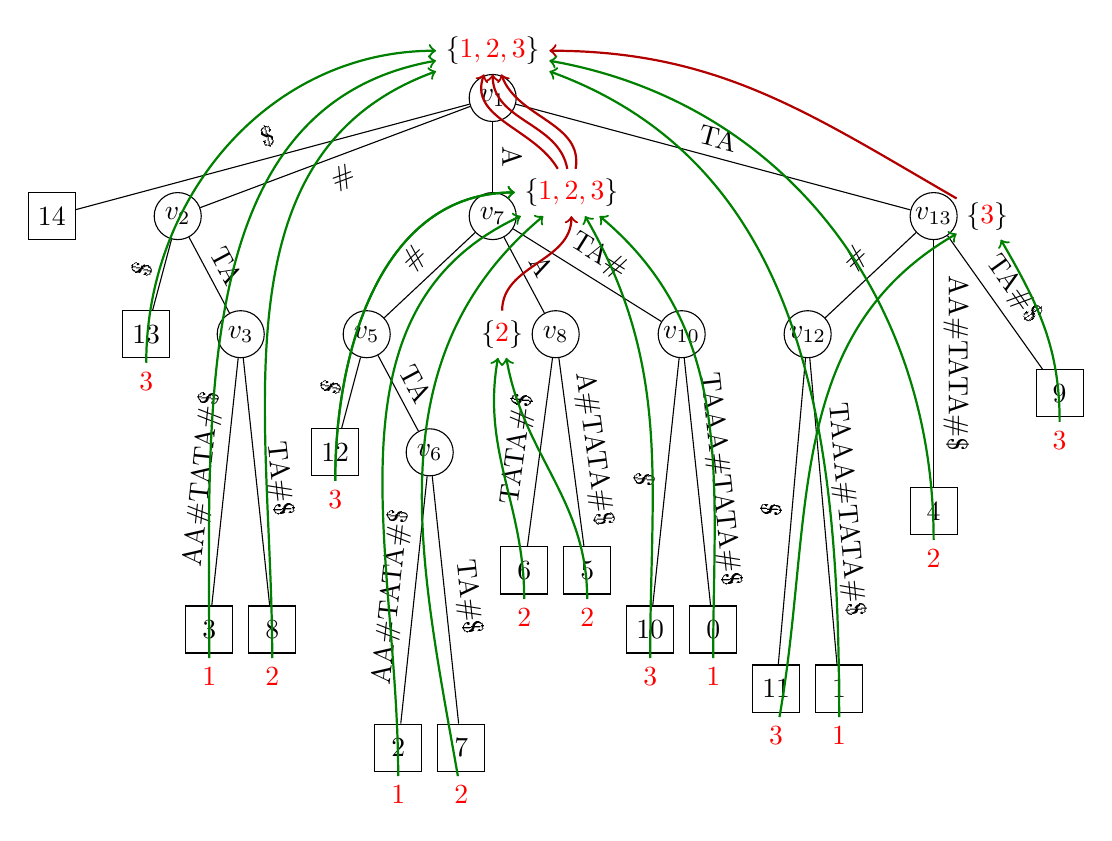
\begin{tikzpicture}[x={(4mm, 0mm)}, y={(0mm, 15mm)}]
  \tikzstyle{vertex}=[draw, minimum size=17pt, inner sep=0pt]

\node[vertex, circle] (v1) at (1, 0) {$v_1$};
\node (l1) at (1, 0.4) {$\{{\color{red}1,2,3}\}$};

\node[vertex, circle] (v2) at (-9, -1) {$v_2$};
\draw (v1) -- (v2) node[below, sloped, pos=0.5] {\#};

\node[vertex, circle] (v3) at (-7, -2) {$v_3$};
\draw (v2) -- (v3) node[above, sloped, pos=0.5] {TA};

\node[vertex, circle] (v7) at (1, -1) {$v_7$};
\node (l7) at (3.5, -0.8) {$\{{\color{red}1,2,3}\}$};
\draw (v1) -- (v7) node[above, sloped, pos=0.5] {A};

\node[vertex, circle] (v5) at (-3, -2) {$v_5$};
\draw (v7) -- (v5) node[above, sloped, pos=0.5] {\#};

\node[vertex, circle] (v6) at (-1, -3) {$v_6$};
\draw (v5) -- (v6) node[above, sloped, pos=0.5] {TA};

\node[vertex, circle] (v8) at (3, -2) {$v_8$};
\node (l8) at (1.3, -2) {$\{{\color{red}2}\}$};
\draw (v7) -- (v8) node[above, sloped, pos=0.5] {A};

\node[vertex, circle] (v10) at (7, -2) {$v_{10}$};
\draw (v7) -- (v10) node[above, sloped, pos=0.5] {TA\#};

\node[vertex, circle] (v13) at (15, -1) {$v_{13}$};
\node (l13) at (16.7, -1) {$\{{\color{red}3}\}$};
\draw (v1) -- (v13) node[above, sloped, pos=0.5] {TA};

\node[vertex, circle] (v12) at (11, -2) {$v_{12}$};
\draw (v13) -- (v12) node[above, sloped, pos=0.5] {\#};

\node[vertex] (s14) at (-13, -1) {$14$};
\draw (v1) -- (s14) node[above, sloped, pos=0.5] {\$};

\node[vertex] (s13) at (-10, -2) {$13$};
\node (d13) at (-10, -2.4) {${\color{red}3}$};
\draw (v2) -- (s13) node[above, sloped, pos=0.5] {\$};

\node[vertex] (s3) at (-8, -4.5) {$3$};
\node (d3) at (-8, -4.9) {${\color{red}1}$};
\draw (v3) -- (s3) node[above, sloped, pos=0.5] {AA\#TATA\#\$};

\node[vertex] (s8) at (-6, -4.5) {$8$};
\node (d8) at (-6, -4.9) {${\color{red}2}$};
\draw (v3) -- (s8) node[above, sloped, pos=0.5] {TA\#\$};

\node[vertex] (s12) at (-4, -3) {$12$};
\node (d12) at (-4, -3.4) {${\color{red}3}$};
\draw (v5) -- (s12) node[above, sloped, pos=0.5] {\$};

\node[vertex] (s2) at (-2, -5.5) {$2$};
\node (d2) at (-2, -5.9) {${\color{red}1}$};
\draw (v6) -- (s2) node[above, sloped, pos=0.5] {AA\#TATA\#\$};

\node[vertex] (s7) at (0, -5.5) {$7$};
\node (d7) at (0, -5.9) {${\color{red}2}$};
\draw (v6) -- (s7) node[above, sloped, pos=0.5] {TA\#\$};

\node[vertex] (s6) at (2, -4) {$6$};
\node (d6) at (2, -4.4) {${\color{red}2}$};
\draw (v8) -- (s6) node[above, sloped, pos=0.5] {TATA\#\$};

\node[vertex] (s5) at (4, -4) {$5$};
\node (d5) at (4, -4.4) {${\color{red}2}$};
\draw (v8) -- (s5) node[above, sloped, pos=0.5] {A\#TATA\#\$};

\node[vertex] (s10) at (6, -4.5) {$10$};
\node (d10) at (6, -4.9) {${\color{red}3}$};
\draw (v10) -- (s10) node[above, sloped, pos=0.5] {\$};

\node[vertex] (s0) at (8, -4.5) {$0$};
\node (d0) at (8, -4.9) {${\color{red}1}$};
\draw (v10) -- (s0) node[above, sloped, pos=0.5] {TAAA\#TATA\#\$};

\node[vertex] (s11) at (10, -5) {$11$};
\node (d11) at (10, -5.4) {${\color{red}3}$};
\draw (v12) -- (s11) node[above, sloped, pos=0.5] {\$};

\node[vertex] (s1) at (12, -5) {$1$};
\node (d1) at (12, -5.4) {${\color{red}1}$};
\draw (v12) -- (s1) node[above, sloped, pos=0.5] {TAAA\#TATA\#\$};

\node[vertex] (s4) at (15, -3.5) {$4$};
\node (d4) at (15, -3.9) {${\color{red}2}$};
\draw (v13) -- (s4) node[above, sloped, pos=0.5] {AA\#TATA\#\$};

\node[vertex] (s9) at (19, -2.5) {$9$};
\node (d9) at (19, -2.9) {${\color{red}3}$};
\draw (v13) -- (s9) node[above, sloped, pos=0.5] {TA\#\$};


  \draw[green!50!black, thick, ->] (d13) to[out=90, in=180] (l1);
  \draw[green!50!black, thick, ->] (d3) to[out=90, in=190] (l1);
  \draw[green!50!black, thick, ->] (d8) to[out=90, in=200] (l1);
  \draw[green!50!black, thick, ->] (d12) to[out=90, in=180] (l7);
  \draw[green!50!black, thick, ->] (d2) to[out=90, in=205] (l7);
  \draw[green!50!black, thick, ->] (d7) to[out=100, in=220] (l7);
  \draw[green!50!black, thick, ->] (d12) to[out=90, in=180] (l7);
  \draw[green!50!black, thick, ->] (d6) to[out=90, in=260] (l8);
  \draw[green!50!black, thick, ->] (d5) to[out=90, in=280] (l8);
  \draw[red!70!black, thick, ->] (l8) to[out=90, in=270] (l7);
  \draw[red!70!black, thick, ->] (l7) to[out=120, in=250] (l1);
  \draw[red!70!black, thick, ->] (l7) to[out=100, in=270] (l1);
  \draw[red!70!black, thick, ->] (l7) to[out=80, in=290] (l1);
  \draw[red!70!black, thick, ->] (l13) to[out=150, in=0] (l1);
  \draw[green!50!black, thick, ->] (d10) to[out=90, in=300] (l7);
  \draw[green!50!black, thick, ->] (d0) to[out=90, in=320] (l7);
  \draw[green!50!black, thick, ->] (d11) to[out=80, in=210] (l13);
  \draw[green!50!black, thick, ->] (d1) to[out=90, in=340] (l1);
  \draw[green!50!black, thick, ->] (d4) to[out=90, in=350] (l1);
  \draw[green!50!black, thick, ->] (d9) to[out=90, in=300] (l13);
\end{tikzpicture}

    \caption{The suffix tree from Figure~\ref{fig:singleTermFrequencySuffixTree} with added arrows between document ids. The red arrows have weight at least $2$.}
    \label{fig:singleTermFrequencySuffixTreeDocumentArrows}
  \end{figure}

  We now have the index to answer queries. Consider a query $q$. We need to find the locus for $q$. Again this is the first node $v$, such that the path to $v$ is prefixed by $q$. Then we observe:
  \begin{itemize}
    \item Per document $i$ there is at most one arrow leaving $v$'s subtree upwards. For each of these pointers we associate a weight: For a pointer of document id $i$, the weight is equal to the number of times document $i$ appears in the subtree of $v$.
    \item The pointer of document $i$ leaving the locus $v$ has the biggest weight among all pointers for document $i$ in $v$'s subtree.
    \item Enumerating all the pointers leaving $v$'s subtree is equivalent to document listing. Top-$k$ frequency corresponds to retrieving the $k$ heaviest pointers (and respectively their corresponding documents).
  \end{itemize}

  % TODO (pjungeblut): This forward references to orthogonal range queries.
  %                    Maybe this chapter should be moved in front of the
  %                    document retrieval chapter. If fixed, remove the note
  %                    that the solution comes "later".
  We will now describe how the problem to find the heaviest pointers can be mapped to an orthogonal range queries problem. This problem can then efficiently be solved with later method.

  From now on we will only consider arrows with a weight at least ~$2$. In Figure~\ref{fig:singleTermFrequencySuffixTreeDocumentArrows} this is the red subset of the arrows. All other (green) arrows correspond to documents where a query appears only once. If our method considering only the heavy arrows returns less than $k$ documents, we can use the classical document listing structure to find more documents.

  Each pointer is assigned a $(x,y)$-coordinate. For this we need a bitvector~$H$ similar to the one used for document listing. It is generated by first writing~$n$~$1$s and then inserting a~$0$ right before the $i$-th~$1$ per upward arrow leaving node~$v_i$. Obviously the~$0$s in~$H$ correspond to the pointers and the pointer corresponding to the~$i$-th~$0$ gets~$x$-coordinate~$i$. The~$y$-coordinate is the depth of the target node of the pointer. In our example we get the values in Table~\ref{tbl:topKPointerCoordinates}. The points are plotted into a grid in Figure~\ref{fig:singleTermFrequencyPlot}.
  \begin{table}[htb]
    \centering
    \begin{tabular}{rcl}
      $H$           & $=$ & \texttt{1~1~1~1~1~1~0~0~0~1~0~1~1~1~1~1~0~1~1~1} \\
      $\mathcal{D}$ & $=$ & \texttt{~~~~~~~~~~~~1~2~3~~~2~~~~~~~~~~~3} \\
      $x$           & $=$ & \texttt{~~~~~~~~~~~~0~1~2~~~3~~~~~~~~~~~4} \\
      $y$           & $=$ & \texttt{~~~~~~~~~~~~0~0~0~~~1~~~~~~~~~~~0} \\
      $w$           & $=$ & \texttt{~~~~~~~~~~~~2~3~2~~~2~~~~~~~~~~~2}
    \end{tabular}
    \caption{The mapping of pointers to coordinates for the example suffix tree in Figure~\ref{fig:singleTermFrequencySuffixTreeDocumentArrows}.}
    \label{tbl:topKPointerCoordinates}
  \end{table}

  \begin{figure}[htb]
    \centering
    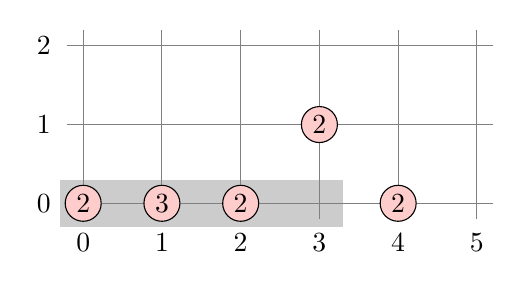
\begin{tikzpicture}
  \tikzstyle{vertex}=[draw, minimum size=13pt, inner sep=0pt]

  \fill[black!20!white] (-0.3, -0.3) -- (3.3, -0.3) -- (3.3, 0.3) -- (-0.3, 0.3) -- cycle;

  \foreach \x in {0, 1, ..., 5} {
    \draw[black!50!white] (\x, -0.2) -- (\x, 2.2);
    \node (x\x) at (\x, -0.5) {$\x$};
  }
  \foreach \y in {0, 1, 2} {
    \draw[black!50!white] (-0.2, \y) -- (5.2, \y);
    \node (y\y) at (-0.5, \y) {$\y$};
  }

  \node[vertex, circle, fill=red!20!white] (p1) at (0, 0) {$2$};
  \node[vertex, circle, fill=red!20!white] (p2) at (1, 0) {$3$};
  \node[vertex, circle, fill=red!20!white] (p3) at (2, 0) {$2$};
  \node[vertex, circle, fill=red!20!white] (p4) at (3, 1) {$2$};
  \node[vertex, circle, fill=red!20!white] (p5) at (4, 0) {$2$};
\end{tikzpicture}

    \caption{The points corresponding to the pointers with weight at least two plotted into a $2$-dimensional grid. The shaded area corresponds to the query range $[0, 3] \times [0, 0]$}
    \label{fig:singleTermFrequencyPlot}
  \end{figure}

  Assume the query $q = \texttt{A}$ and \proc{Backward Search} returns a suffix array interval $[l,r] = [4,10]$ for it. These are the positions of the leftmost and rightmost leaves descending form locus $v = v_7$ (note that $v$ is not computed and not known). Via two select queries interval $[l,r]$ can be mapped to an interval $[l',r'] = [0,3]$ in the $x$-coordinates. We extract the positions of the zeros in $H$ in $[l,r]$ as shown in Algorithm~\ref{alg:singleTermFrequencyMapInterval}. For the $y$-coordinates the lower bound is always $0$. For the upper bound we remember that the $y$-coordinate of the plotted points is the depth of the target node and that we only want to find arrows ending above the locus. Therefore we can take the length $\vert q \vert - 1$ as the upper $y$-coordinate. We reduced the query operation to a $3$-sided range query for the $k$ heaviest points in $[l', r'] \times [0, \vert q \vert - 1]$. This can be solved with the known range query methods. For our example the query range is shown shaded in Figure~\ref{fig:singleTermFrequencyPlot}.

  \begin{algorithm}[htb]
    \begin{codebox}
      \Procname{$\proc{Map-Interval}([l,r])$}
      \li $[l', r'] \gets [0, -1]$
      \li \If $l > 0$
          \Then
      \li   $l' \gets \proc{Select}_1(l - 1, H) - (l - 1)$
          \End
      \li \If $r > 0$
          \Then
      \li   $r' \gets \proc{Select}_1(r - 1, H) - r$
          \End
      \li \Return $[l', r']$
    \end{codebox}
    \caption{Maps a suffix array interval $[l,r]$ to an $x$-interval $[l',r']$.}
    \label{alg:singleTermFrequencyMapInterval}
  \end{algorithm}
\end{Proof}

At last, an optimal solution is known but is not covered in this document.

\begin{Theorem}
  The top-$k$ documents can be found in time $\mathcal{O}(m + k)$ query time in $\mathcal{O}(n \log n)$ bits space (Navarro \& Nekrich \cite{Navarro2012} based on framework by Hon \cite{Hon2014}).
\end{Theorem}
